\documentclass[letterpaper]{article}
\usepackage[margin=1in]{geometry} % Sets page size and 1-inch margins
\usepackage[svgnames,dvipsnames]{xcolor}   % For a wider range of colors

\usepackage{amsmath} % For math symbols
\usepackage{array}   % For advanced column specifications
\usepackage{tabularx}% For tables with auto-expanding columns
\usepackage{tikz}
\usetikzlibrary{
    positioning,      % For placing nodes relative to each other (e.g., below=of)
    shapes.geometric, % For shapes like ellipses
    arrows.meta,      % For advanced arrow tips (e.g., Stealth)
    decorations.pathmorphing, % For snake/squiggly lines
    calc              % For coordinate calculations
}

% --- GLOBAL STYLE DEFINITIONS FOR DFD ---
\tikzset{
    % A shape for logical connectives
    connective_node/.style={
        rectangle, rounded corners=5pt, draw=black!80, fill=black!10,
        inner sep=5pt, thick, align=center
    },
    % A shape for Introduction Rules
    intro_rule_node/.style={
        rectangle, rounded corners=5pt, draw=black!80, fill=Teal!20,
        inner sep=5pt, thick, align=center
    },
    % A shape for Elimination Rules
    elim_rule_node/.style={
        rectangle, rounded corners=5pt, draw=black!80, fill=BurntOrange!20,
        inner sep=5pt, thick, align=center
    },
    % A shape for abstract propositions
    proposition_node/.style={
        ellipse, draw=black!80, fill=Violet!15,
        inner sep=3pt, align=center
    },
    % A shape for concrete proof terms
    proof_node/.style={
        ellipse, draw=black!80, fill=Green!15,
        inner sep=3pt, align=center
    },
    % Arrow styles with color
    input_arrow/.style={-Stealth, solid, thick, draw=blue!70!black},
    output_arrow/.style={double, double distance=1.5pt, -Stealth, solid, thick, draw=ForestGreen!80!black},
    proves_arrow/.style={-Stealth, decorate, decoration={snake, segment length=6pt, amplitude=1pt}, thick, draw=orange!90!black}
}

\begin{document}

\begin{figure}[h!]
\centering
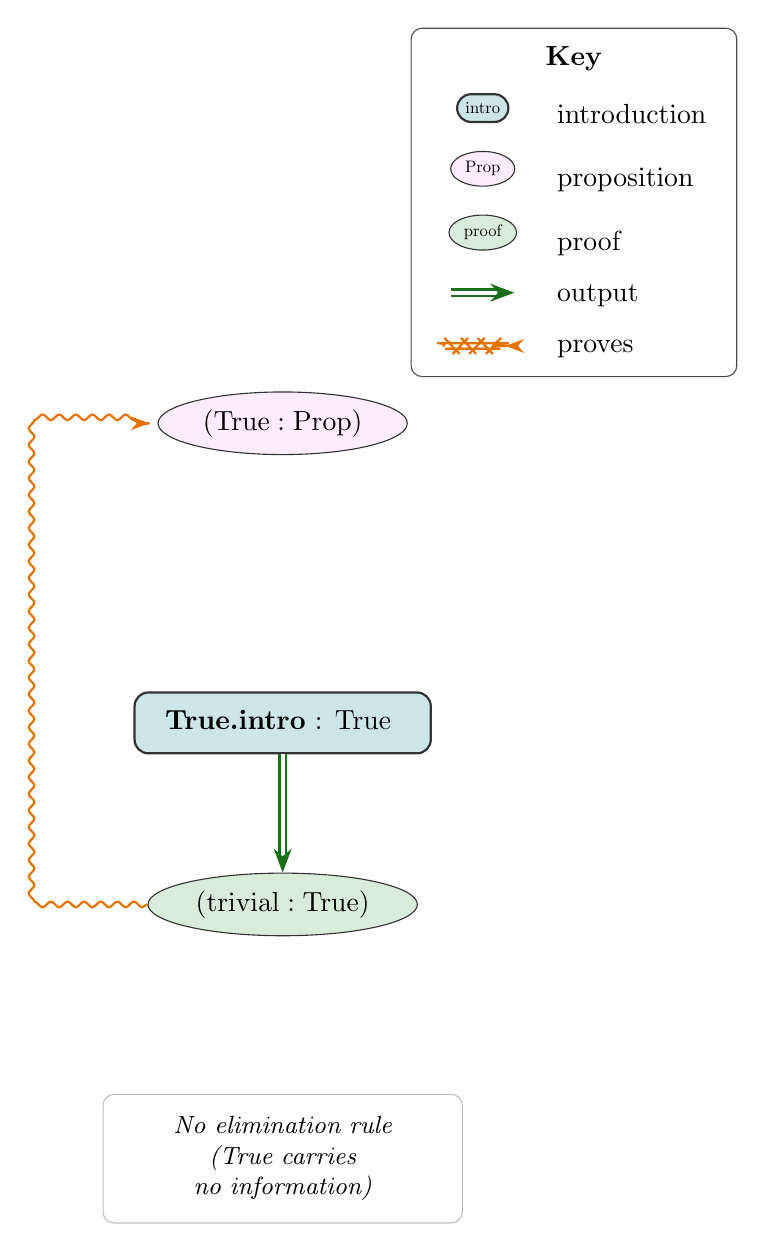
\begin{tikzpicture}[node distance=2cm and 2.5cm]

% --- NODE DEFINITIONS FOR "TRUE" DIAGRAM ---

% Top proposition layer
\node[proposition_node] (True_prop) {$(\text{True} : \text{Prop})$};

% Introduction layer - the trivial proof
\node[intro_rule_node, below=3cm of True_prop] (true_intro) {
    \begin{tabular}{c}
    \textbf{True.intro} : True
    \end{tabular}
};

\node[proof_node] (trivial_proof) [below=1.5cm of true_intro] {$(\text{trivial} : \text{True})$};

% Note about elimination
\node[draw=gray!50, rounded corners, inner sep=8pt, below=2cm of trivial_proof, text width=4cm, align=center, font=\small\itshape] (no_elim) {
    No elimination rule\\
    (True carries no information)
};

% --- EDGE ROUTING ---

% Introduction flow
\draw[output_arrow] (true_intro) -> (trivial_proof);

% Proves arrow - routed around the diagram
\coordinate (outset_point) at ($(True_prop.west)+(-1.5cm,0)$);
\draw[proves_arrow, shorten >=3pt] (trivial_proof.west) -- (outset_point |- trivial_proof.west) -- (outset_point |- True_prop.west) -- (True_prop.west);

% --- LEGEND ---
\node (legend) [draw=black!70, rounded corners, inner sep=5pt, above right=0.3cm and 0.5cm of True_prop] {
    \begin{tabular}{cl}
    \multicolumn{2}{c}{\textbf{Key}} \\[1.5ex]
    \tikz{\node[intro_rule_node, scale=0.6] {intro};} & introduction \\[1.5ex]
    \tikz{\node[proposition_node, scale=0.6] {Prop};} & proposition \\[1.5ex]
    \tikz{\node[proof_node, scale=0.6] {proof};} & proof \\[1.5ex]
    \tikz{\draw[output_arrow] (0,0.1) -- (0.8,0.1);} & output \\[1.5ex]
    \tikz{\draw[proves_arrow] (0,0.1) -- (0.8,0.1);} & proves \\
    \end{tabular}
};

\end{tikzpicture}
\caption{The algebra of True. The proposition True represents a trivially provable statement
in constructive logic. It has a single introduction rule \texttt{True.intro} that produces 
the canonical proof term \texttt{trivial}. True has no elimination rule because it carries 
no computational information - knowing that True is provable tells us nothing new. In the 
propositions-as-types correspondence, True corresponds to the unit type with a single 
inhabitant. This makes True the terminal object in the category of propositions under 
logical implication.}\label{fig:tikz_diagram_true}
\end{figure}

\end{document}